\normaltrue \difficilefalse \tdifficilefalse
\correctiontrue
%\UPSTIidClasse{11} % 11 sup, 12 spé
%\newcommand{\UPSTIidClasse}{11}

\exer{Machine de rééducation SysReeduc $\star$ \label{B2:07:47}}
\setcounter{numques}{0}
\UPSTIcompetence[2]{B2-07}
\index{Compétence B2-07}
\index{Machine de rééducation SysReeduc}
\index{Schéma-blocs}
\ifcorrection
\else
\textbf{Pas de corrigé pour cet exercice.}
\fi



\ifprof
\else
On propose une modélisation par schéma-blocs dans la figure suivante. 
\begin{figure}[H]
\centering
{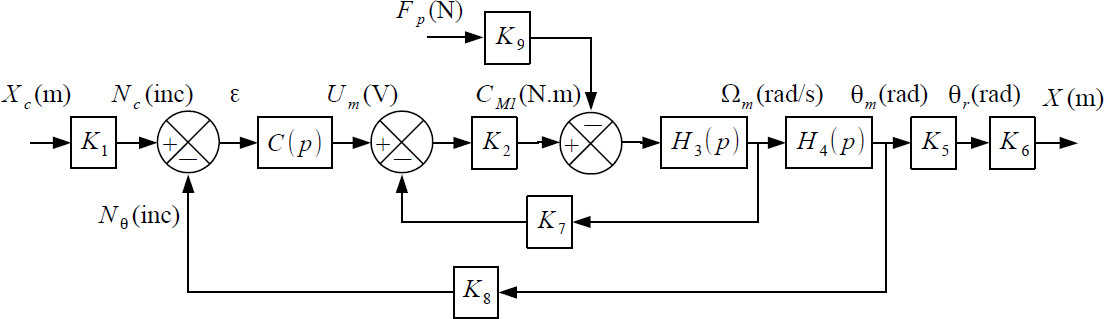
\includegraphics[width=\linewidth]{47_01}}
%\caption{ \label{fig_47_01}}
\end{figure}




Le moteur à courant continu est régi par les équations suivantes :
$ u_m(t)=e(t)+Ri(t)$, $e(t)=k_e\omega_m(t)$ et $C_{M1}(t)=k_t i(t)$. 

Une étude dynamique a mené à l'équation suivante : 
$$\left(M+m\right)r\rho_1 \dot{\omega}_m(t)=\dfrac{C_{M1}(t)}{\rho_1 r}-F_p(t)$$ avec : $M$ la masse du chariot et $m$ la masse du support de pied, $\rho_1=\dfrac{1}{10}$ le rapport de réduction du réducteur, $r=\SI{46,1}{mm}$ le rayon de la poulie du transmetteur poulie--courroie, $C_{M1}(t)$ le couple délivré par le moteur et $F_p(t)$ l'effort délivré par le patient sur le support 3. 

Le codeur incrémental possède 500 fentes équiréparties. Deux émetteurs-récepteurs positionnés en quadrature permettent de mesurer l'information. 
\fi

\question{À partir des équations proposées, déterminer les fonctions de transfert $K_1$, $K_2$, $H_3(p)$, $H_4(p)$,  $K_5$, $K_6$, $K_7$, $K_8$ et $K_9$.}
\ifprof
%\begin{corrige}
~\\
On a :
\begin{itemize}
\item $ u_m(t)=e(t)+Ri(t) \Rightarrow  U_m(p)=E(p)+RI(p) $ et $C_{M1}(p)=k_t I(p)$ donc $K_2 = \dfrac{k_t}{R}$;
\item $E(p)=k_e\Omega_m(p)$ et donc $K_7 = k_e$;
\item $\left(M+m\right)r\rho_1 p\Omega_m(p)=\dfrac{C_{M1}(p)}{\rho_1 r}-F_p(p) \Leftrightarrow\left(M+m\right)r^2\rho_1^2 p\Omega_m(p)=C_{M1}(p)-\rho_1 rF_p(p) $ et donc $K_9 = \rho_1 r$ et $H_3(p)=\dfrac{1}{\left(M+m\right)r^2\rho_1^2 p}$;
\item  $H_4(p)$ permet d'obtenir une position à partir d'une vitesse. Il s'agit donc d'un intégrateur et $H_4(p)=\dfrac{1}{p}$; 
\item un codeur incrémental avec 1 émetteur-récepteur permet de détecter les fentes et les << non fentes >> donc ici 1000 informations par tour. Avec un second émetteur, on double la résolution soit 2000 informations pour un tour soit $K_8  = \dfrac{2000}{2\pi}$;
\item en utilisant le réducteur et le poulie courroie, on a directement $K_5=\rho_1$ et $K_6=r$ (à convertir en mètres);
\item enfin, $K_1$ convertit des mètres en incréments. $X_c$ est la consigne que doit respectée $X$. Pour avoir un asservissement précis, il faut donc $\varepsilon = 0$ et $X=X_c$ soit $\varepsilon = 0 = K_1 X_C - K_8 \theta_m = K_1 X_C - K_8 \dfrac{X}{K_5 K_6}$. Au final, $K_1 =\dfrac{K_8}{K_5 K_6}$.
\end{itemize}
%\end{corrige}
\else
\fi


\question{Montrer que le schéma-blocs peut être mis sous la forme suivante. On exprimera $A$, $B$ et $D$ en fonction des paramètres du système $r$, $\rho_1$, $k_t$, $k_e$, $R$, $M$, $m$ et $K_8$. }
\ifprof
%\begin{corrige}~\\
D'une part,

$X(p)=\left(\left(X_C(p)-X(p)\right)C(p)-F_P(p) D \right)\dfrac{A}{p\left(Bp+1\right)}$

$X(p)=\dfrac{A\left(X_C(p)-X(p)\right)C(p)}{p\left(Bp+1\right)}- \dfrac{AF_P(p) D}{p\left(Bp+1\right)}$

$\Leftrightarrow X(p)+\dfrac{AX(p)C(p)}{p\left(Bp+1\right)}=\dfrac{AX_C(p)C(p)}{p\left(Bp+1\right)}- \dfrac{AF_P(p) D}{p\left(Bp+1\right)}$.
$\Leftrightarrow X(p)\left(\dfrac{p\left(Bp+1\right)+AC(p)}{p\left(Bp+1\right)}\right)=\dfrac{AX_C(p)C(p)}{p\left(Bp+1\right)}+ \dfrac{AF_P(p) D}{p\left(Bp+1\right)}$

\fbox{$\Leftrightarrow X(p)=\dfrac{AX_C(p)C(p)}{p\left(Bp+1\right)+AC(p)}- \dfrac{AF_P(p) D}{p\left(Bp+1\right)+AC(p)}$.}


D'autre part, 
$X(p)=\Omega_m(p)H_4(p)K_5K_6$, $U_m(p)=\left(X_c(p)K_1 - \theta_m(p)K_8\right)C(p)$, $\theta_m(p)=\Omega_m(p)H_4(p)$. 

$\Omega_m(p) = \left(\left(U_m(p)-\Omega_m(p) K_7\right)K_2- F_P(p)K_9\right)H_3(p)$

$\Leftrightarrow \Omega_m(p) \left(1+K_7K_2H_3(p)\right)= U_m(p)H_3(p)K_2- F_P(p)H_3(p)K_9$


$X(p)=\left( U_m(p)H_3(p)K_2- F_P(p)H_3(p)K_9 \right)\dfrac{H_4(p)K_5K_6}{1+K_7K_2H_3(p)}$

$\Leftrightarrow X(p)=\left( \left(X_c(p)K_1 - \theta_m(p)K_8\right)C(p)H_3(p)K_2- F_P(p)H_3(p)K_9 \right)\dfrac{H_4(p)K_5K_6}{1+K_7K_2H_3(p)}$

$\Leftrightarrow X(p)=\left( \left(X_c(p)K_1 - X(p)\dfrac{K_8}{K_5K_6}\right)C(p)H_3(p)K_2- F_P(p)H_3(p)K_9 \right)\dfrac{H_4(p)K_5K_6}{1+K_7K_2H_3(p)}$

$\Leftrightarrow X(p)=\left(\left(X_c(p) - X(p)\right)C(p)H_3(p)  K_1K_2- F_P(p)H_3(p)K_9 \right)\dfrac{H_4(p)K_5K_6}{1+K_7K_2H_3(p)}$

$\Leftrightarrow X(p)\left( 1+ C(p)H_3(p)  K_1K_2 \dfrac{H_4(p)K_5K_6}{1+K_7K_2H_3(p)}\right)=\left(X_c(p) C(p)H_3(p)  K_1K_2- F_P(p)H_3(p)K_9 \right)\dfrac{H_4(p)K_5K_6}{1+K_7K_2H_3(p)}$


\fbox{$\Leftrightarrow X(p)\left( 1+K_7K_2H_3(p)+ C(p)H_3(p)  K_1K_2 H_4(p)K_5K_6\right)=\left(X_c(p) C(p)H_3(p)  K_1K_2- F_P(p)H_3(p)K_9 \right)H_4(p)K_5K_6$}.




Par suite, 

$\Leftrightarrow X(p)\left( 1+K_7K_2 \dfrac{1}{\left(M+m\right)r^2\rho_1^2 p} + C(p)\dfrac{1}{\left(M+m\right)r^2\rho_1^2 p}  \dfrac{K_8}{K_5 K_6} K_2 \dfrac{1}{p} K_5K_6\right)=\left(X_c(p) C(p)\dfrac{1}{\left(M+m\right)r^2\rho_1^2 p}  \dfrac{K_8}{K_5 K_6} K_2- F_P(p)\dfrac{1}{\left(M+m\right)r^2\rho_1^2 p} K_9 \right)\dfrac{1}{p}K_5K_6$

$\Leftrightarrow X(p)\left( 1+ \dfrac{ \dfrac{k_ek_t}{R}}{\left(M+m\right)r^2\rho_1^2 p} + C(p)\dfrac{K_8 \dfrac{k_t}{R}}{\left(M+m\right)r^2\rho_1^2 p^2} \right)
=
\left(X_c(p) C(p)\dfrac{K_8}{\left(M+m\right)r^2\rho_1^2 p^2}  \dfrac{k_t}{R}- F_P(p)\dfrac{K_9}{\left(M+m\right)r\rho_1 p^2}  \right)$.

$\Leftrightarrow X(p)
=
X_c(p) C(p)\dfrac{\dfrac{K_8}{\left(M+m\right)r^2\rho_1^2 p^2}  \dfrac{k_t}{R}}{\left( 1+ \dfrac{ \dfrac{k_ek_t}{R}}{\left(M+m\right)r^2\rho_1^2 p} + C(p)\dfrac{K_8 \dfrac{k_t}{R}}{\left(M+m\right)r^2\rho_1^2 p^2} \right)}
- F_P(p)\dfrac{\dfrac{K_9}{\left(M+m\right)r\rho_1 p^2}}{\left( 1+ \dfrac{ \dfrac{k_ek_t}{R}}{\left(M+m\right)r^2\rho_1^2 p} + C(p)\dfrac{K_8 \dfrac{k_t}{R}}{\left(M+m\right)r^2\rho_1^2 p^2} \right)}
$


$\Leftrightarrow X(p)
=
X_c(p) C(p)\dfrac{\dfrac{K_8}{1}  \dfrac{k_t}{R}}{\left( \left(M+m\right)r^2\rho_1^2 p^2+ \dfrac{\left(M+m\right)r^2\rho_1^2 p^2 \dfrac{k_ek_t}{R}}{\left(M+m\right)r^2\rho_1^2 p} + C(p)\dfrac{ \left(M+m\right)r^2\rho_1^2 p^2K_8 \dfrac{k_t}{R}}{\left(M+m\right)r^2\rho_1^2 p^2} \right)}
- F_P(p)\dfrac{\dfrac{K_9}{\left(M+m\right)r\rho_1 p^2}}{\left( 1+ \dfrac{ \dfrac{k_ek_t}{R}}{\left(M+m\right)r^2\rho_1^2 p} + C(p)\dfrac{K_8 \dfrac{k_t}{R}}{\left(M+m\right)r^2\rho_1^2 p^2} \right)}
$


$\Leftrightarrow X(p)
=
X_c(p) C(p)\dfrac{  \dfrac{K_8k_t}{R}}{
 \left(M+m\right)r^2\rho_1^2 p^2
 + p \dfrac{k_ek_t}{R} 
 + C(p)K_8 \dfrac{k_t}{R}
 }
- F_P(p)\dfrac{\dfrac{K_9}{1}}{\left( \left(M+m\right)r\rho_1 p^2+ \dfrac{ \left(M+m\right)r\rho_1 p^2\dfrac{k_ek_t}{R}}{\left(M+m\right)r^2\rho_1^2 p} + C(p)\dfrac{ \left(M+m\right)r\rho_1 p^2K_8 \dfrac{k_t}{R}}{\left(M+m\right)r^2\rho_1^2 p^2} \right)}
$


$\Leftrightarrow X(p)
=
X_c(p) C(p)\dfrac{  \dfrac{K_8k_t}{R}}{
 \left(M+m\right)r^2\rho_1^2 p^2
 + p \dfrac{k_ek_t}{R} 
 + C(p)K_8 \dfrac{k_t}{R}
 }
- F_P(p)\dfrac{K_9}{
 \left(M+m\right)r\rho_1 p^2
 + \dfrac{  pk_ek_t}{Rr\rho_1} 
 + C(p)\dfrac{ K_8 k_t}{Rr\rho_1 } }
$


$\Leftrightarrow X(p)
=
X_c(p) C(p)\dfrac{
\dfrac{K_8k_t}{R}}{
p\dfrac{k_ek_t}{R}\left(\dfrac{R}{k_ek_t}
 \left(M+m\right)r^2\rho_1^2 p
 +  1\right) 
 + C(p)K_8 \dfrac{k_t}{R}
 }
- F_P(p)\dfrac{K_9}{
p\dfrac{  k_ek_t}{Rr\rho_1}\left(
\dfrac{\left(M+m\right) Rr^2\rho_1^2}{  k_ek_t}  p
 + 1\right)
 + C(p)\dfrac{ K_8 k_t}{Rr\rho_1 } }
$



$\Leftrightarrow X(p)
=
X_c(p) C(p)\dfrac{
\dfrac{K_8k_t}{R}}{
p\dfrac{k_ek_t}{R}\left(B p
 +  1\right) 
 + C(p)K_8 \dfrac{k_t}{R}
 }
- F_P(p)\dfrac{K_9}{
p\dfrac{  k_ek_t}{Rr\rho_1}\left(
B  p
 + 1\right)
 + C(p)\dfrac{ K_8 k_t}{Rr\rho_1 } }
$

$\Leftrightarrow X(p)
=
X_c(p) C(p)\dfrac{
\dfrac{K_8k_t}{R}}{
p\dfrac{k_ek_t}{R}\left(B p
 +  1\right) 
 + C(p)K_8 \dfrac{k_t}{R}
 }
- F_P(p)\dfrac{K_9}{
p\dfrac{  k_ek_t}{Rr\rho_1}\left(
B  p
 + 1\right)
 + C(p)\dfrac{ K_8 k_t}{Rr\rho_1 } }
$

$\Leftrightarrow X(p)
=
X_c(p) C(p)\dfrac{
\dfrac{R}{k_ek_t}\dfrac{K_8k_t}{R}}{
p\left(B p +  1\right) 
 + C(p)K_8 \dfrac{k_t}{R} \dfrac{R}{k_ek_t}
 }
- F_P(p)\dfrac{K_9\dfrac{Rr\rho_1}{  k_ek_t}}{
p\left(
B  p
 + 1\right)
 + C(p)\dfrac{Rr\rho_1}{  k_ek_t}\dfrac{ K_8 k_t}{Rr\rho_1 } }
$

$\Leftrightarrow X(p)
=
X_c(p) C(p)\dfrac{
\dfrac{K_8}{k_e}}{
p\left(B p +  1\right) 
 + C(p) \dfrac{K_8 }{k_e}
 }
- F_P(p)\dfrac{K_9\dfrac{Rr\rho_1}{  k_ek_t}}{
p\left(
B  p
 + 1\right)
 + C(p)\dfrac{K_8}{  k_e} }
$



$\Leftrightarrow X(p)
=
X_c(p) C(p)\dfrac{
\dfrac{K_8}{k_e}}{
p\left(B p +  1\right) 
 + C(p) \dfrac{K_8 }{k_e}
 }
- F_P(p)\dfrac{ \dfrac{K_8}{  k_e} \dfrac{  k_e}{K_8}K_9\dfrac{Rr\rho_1}{  k_ek_t}}{
p\left(
B  p
 + 1\right)
 + C(p)\dfrac{K_8}{  k_e} }
$



On a donc $A=\dfrac{K_8}{k_e}$, $B=\dfrac{R\left(m+M\right)r^2\rho_1^2}{k_ek_t}$ et 
$D = \dfrac{ K_9 Rr\rho_1}{  K_8k_t}$.
%$D=\dfrac{r^2\rho_1^2R}{K_8k_t}$.
%\end{corrige}
\else
\fi

\ifprof
\else
\footnotesize
\noindent
\begin{tabular}{|p{\linewidth}|}
\hline
\begin{enumerate}
\item ...
\begin{itemize}
\item  $K_2 = \dfrac{k_t}{R}$;
\item $K_7 = k_e$;
\item  $K_9 = \rho_1 r$ et $H_3(p)=\dfrac{1}{\left(M+m\right)r^2\rho_1^2 p}$;
\item   $H_4(p)=\dfrac{1}{p}$; 
\item $K_8  = \dfrac{2000}{2\pi}$;
\item t $K_5=\rho_1$ et $K_6=r$ (à convertir en mètres);
\item  $K_1 =\dfrac{K_8}{K_5 K_6}$.
\end{itemize}
\item $A=\dfrac{K_8}{k_e}$, $B=\dfrac{R\left(m+M\right)r^2\rho_1^2}{k_ek_t}$ et 
$D = \dfrac{ K_9 Rr\rho_1}{  K_8k_t}$
\end{enumerate} \\ \hline
\end{tabular}
\normalsize
\begin{figure}[H]
\centering
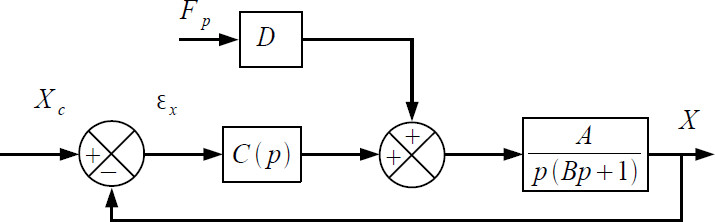
\includegraphics[width=\linewidth]{47_02}
%\caption{ \label{fig_47_02}}
\end{figure}
\fi







\ifprof
\else
\begin{flushright}
\footnotesize{Corrigé  voir \ref{B2:07:47}.}
\end{flushright}%
\fi